\documentclass[a4paper,12pt]{article}        
\usepackage[utf8]{inputenc}         
\usepackage[french]{babel}  
\usepackage[T1]{fontenc} %encodage de la police 
\usepackage[top=2cm,bottom=2cm,left=2cm,right=2cm]{geometry} %marges
\usepackage{graphicx} %affichage des images    
\usepackage{hyperref} %pour les liens
\usepackage[ruled, vlined, linesnumbered, french, onelanguage]{algorithm2e} %pour afficher un algorithme
\usepackage{listings} %pour afficher des lignes de code
\usepackage{xcolor} %ajoute de la couleur aux lignes de code
\usepackage{float} %pour placer correctement les images
\usepackage[linesnumbered, ruled, french, onelanguage]{algorithm2e}
\usepackage{amsmath}

\title{\textbf{Tables arc-en-ciel}}
\author{TRANSON Alexandre, RABOT Valentin, MAHIER Awen, FAUQUETTE Mael \\ \\ L3 Informatique Groupe 3A}
\date{\today}
\pagenumbering{gobble}

\begin{document}

\maketitle
\begin{figure}[h]
\centering
\includegraphics[scale=1]{img/LogoUniCaen.png}
\end{figure}

\newpage
\tableofcontents
\newpage

\section{Introduction}
\subsection{Description générale du projet}
Il s'agit d'une table arc-en-ciel programmé en Java, dotée d'une interface graphique, qui consiste à réduire les temps de calcul pour retrouver un mot de passe original au prix d'un coût en espace. Le hash est au cœur de ce système, étant utilisé pour l'identification des mots de passe originaux à partir de leurs hash correspondants.

\subsection{Présentation du plan du rapport}
Maintenant que nous avons introduit le sujet sur lequel porte notre projet et que nous avons pu lister les divers objectifs à atteindre, nous allons maintenant expliquer le plan global que suivra ce rapport de projet afin d'exposer notre projet de la manière la plus claire possible.\\\\Dans un premier temps nous allons voir chacun des objectifs fixés un peu plus en détails et nous allons expliquer plus concrètement en quoi consistent-ils. Ensuite, nous verrons comment ces objectifs ont pu être traités dans d'autres projets et essayer de s'en inspirer ou de voir une manière différente de répondre à certaines contraintes.\\\\Suite à cela nous expliquerons les principales fonctionnalités à implémenter et comment nous nous sommes organisés au sein de notre groupe afin de mener à bien l'implémentation de ces dernières.\\\\Une fois notre organisation présentée nous verrons les divers éléments techniques auxquels nous devrons apporter des réponses au sein de ce projet. Puis nous verrons comment nous avons élaboré les divers algorithmes imaginés et utilisés dans notre projet. Pour terminer avec cette partie nous verrons comment sont organisées les diverses données utilisées dans nos algorithmes.\\\\Pour la suite du rapport nous exposerons l'architecture de notre projet avec notamment le diagramme des classes.\\\\Ensuite nous testerons notre programme afin d'explorer les divers angles d'usages de notre projet et expliquer quelles sont les données renvoyées et leur utilité.\\\\Pour finir ce rapport nous conclurons par un récapitulatif de la problématique, des fonctionnalités ainsi que des résultats de notre projet puis par la proposition d'axes d'amélioration qui pourraient être à réfléchir à l'avenir.

\pagenumbering{arabic}

\section{Objectifs du projet}
\subsection{Problématique du projet}
Afin de produire ce projet nous avons suivi une ligne conductrice basée sur une problématique bien précise, \textbf{comment créer une table arc-en-ciel fonctionnelle et optimisée ?} En effet, nous avions pour principaux objectifs :
\begin{itemize}
    \item Générer une base synthétique de mots de passe hachés
    \item Implémenter une table arc-en-ciel (paramétrable en termes de couleurs)
    \item Implémenter des optimisations de la table arc-en-ciel
\end{itemize}
Nous allons voir plus en détail ces différents points dans les prochaines parties.

\subsection{Description des points-clés et des grandes étapes}
Voici les étapes importantes que nous avons suivis :\newline
Étape 1 : L'analyse des besoins, identification des objectifs du projet, ainsi que des fonctionnalités qu'on souhaité inclure.\newline
Étape 2 : Implémentation des fonctionnalités de base, telle que le hachage, le stockage de mot de passe dans un fichier, etc.\newline
Étape 3 : Développement des fonctionnalités principales, telle que la comparaison de hachages, la recherche de mots de passe, etc.\newline
Étape 4 : Tests et débogage, en effectuant des tests unitaires de l'application afin de vérifier son bon fonctionnement.\newline
Étape 5 : Les optimisations et les améliorations, afin d'avoir de meilleures performances.\newline 

\subsection{Description de travaux existants sur le même sujet}
Le site \href{https://freerainbowtables.com/}{freerainbowtables.com} propose une variété de tables arc-en-ciel pour différents types de hachage, tels que NTLM, SHA-1, MD5, LM, etc..., avec des capacités de cracking allant jusqu'à plusieurs téraoctets en fonction du type de hachage et de la longueur du mot de passe. Ces tables sont souvent disponibles gratuitement en téléchargement via des liens BitTorrent.
\begin{figure}[H]
\centering
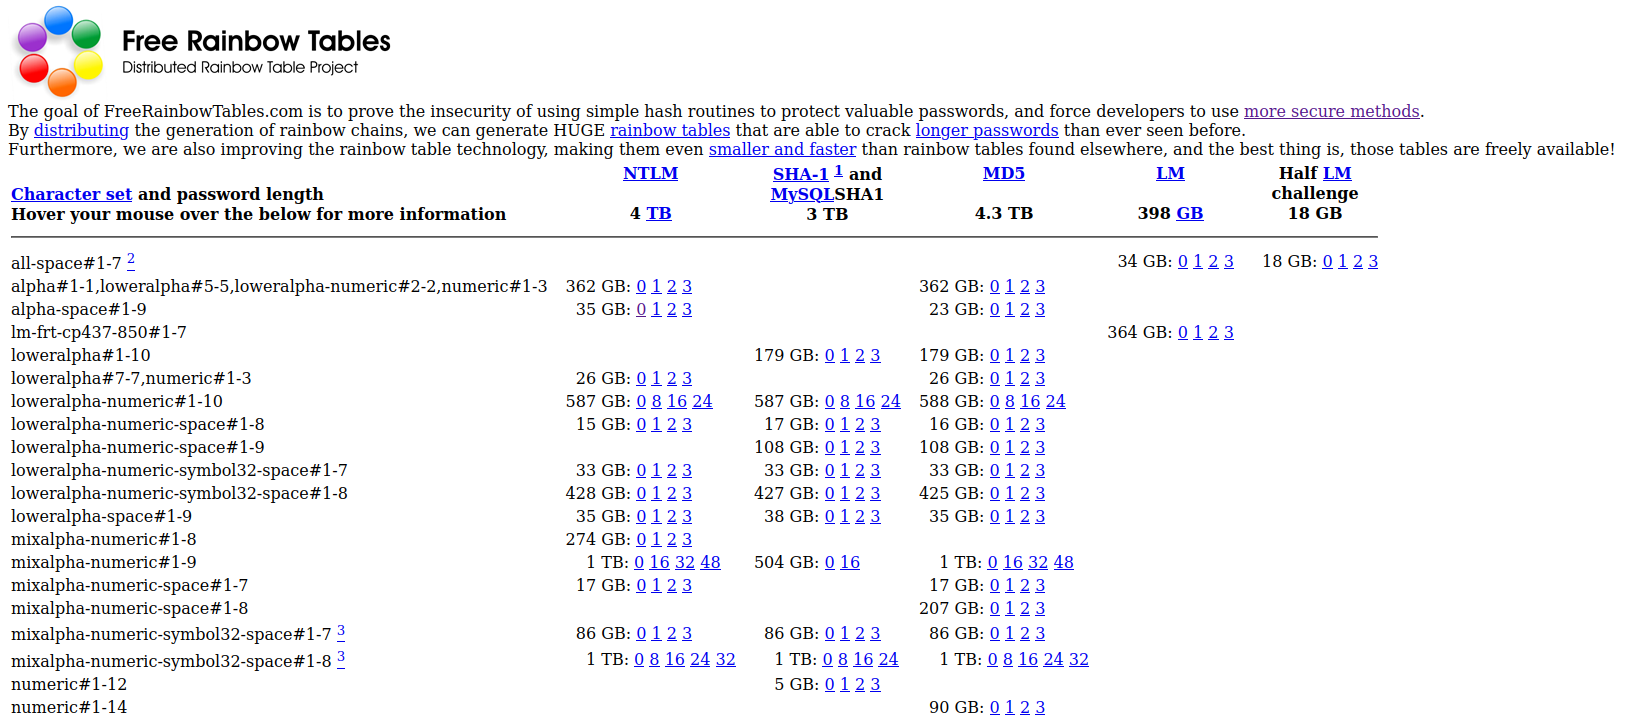
\includegraphics[height=8cm]{img/freerainbowtables.png}
\caption{Page d'accueil du site freerainbowtables.com}
\end{figure}

\section{Fonctionnalités implémentées}
\subsection{Fonctionnement}

\begin{figure}[H]
\centering
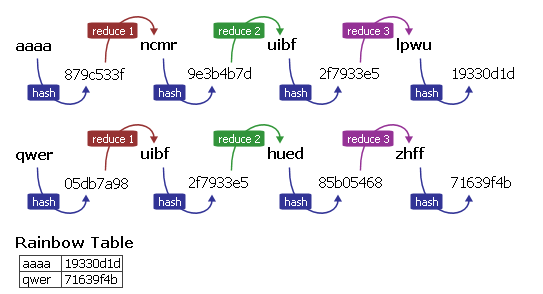
\includegraphics[height=10cm]{img/fonctionnement.png}
\caption{Génération d’une rainbow table}
\end{figure}

On part d'un mot de passe puis on le hash, le hachage est une fonction qui prend en entrée un mot de passe et produit en sortie une empreinte numérique, appelée le hash. Cette fonction est conçue de telle sorte que deux ensembles de données différents produisent généralement des hashs différents et qu'il est difficile de retrouver le mot de passe à partir du hash. Cependant, plusieurs entrées peuvent générer le même hash (collision de hachage), ce qui est un aspect à considérer lors de l'utilisation de tables arc-en-ciel pour retrouver le mot de passe à partir d'un hash on utilise la réduction qui est le processus inverse du hachage. Elle consiste à prendre un hash et à le convertir en une valeur. Cette valeur réduite est utilisée comme point de départ pour générer une nouvelle chaîne de données, qui sera ensuite hachée à nouveau. La fonction de réduction est conçue pour produire une distribution uniforme des valeurs réduites.
\subsection{Description des fonctionalités}
\subsubsection{Génération des mots de passe}
    \begin{algorithm}[H]
        \caption{Algorithme de génération de mot de passe}
        \SetKwInOut{Output}{Sortie}
        \Output{Un mot de passe généré "mdp"}
        $\text{seed} \gets 0$\;
        \For{$c$ \textbf{in} $\text{this.hashpw.toCharArray()}$}{
            $\text{seed} \gets 31L \times \text{seed} + c$\;
        }
        $\text{generator} \gets$ \textbf{new} Random$(\text{seed})$\;
        $\text{alphabet} \gets \text{"abcdefghijklmnopqrstuvwxyzABCDEFGHIJKLMNOPQRSTUVW}$ \text{XYZ0123456789[]!()*+,-./:;<>=|?"}\;
        $n \gets \text{generator.nextInt(32) + 8}$\;
        $\text{mdp} \gets ""$\;
        \For{$z \gets 0$ \textbf{to} $n$}{
            $c \gets \text{alphabet.charAt(generator.nextInt(alphabet.length()))}$\;
            $\text{mdp} \gets \text{mdp} + c$\;
        }
        \textbf{return} mdp\;
    \end{algorithm}

    On calcul une "seed" (graine) en parcourant chaque caractère d'un hash donné qui sera utilisée pour créer un objet Random afin de générer des nombres aléatoires. Puis une longueur 'n' est sélectionnée pour le mot de passe entre 8 et 32 caractères, ensuite on itère n fois pour choisir aléatoirement un caractère d'une chaîne contenant les lettres de l'alphabet en minuscule et majuscule, les chiffres et quelques caractères spéciaux et l'ajouter au mot de passe.
    
    \subsubsection{Stockage des mots de passe}
    Ils sont stockés dans un fichier texte avec comme première ligne la profondeur de la compression et la liste des fonctions de réductions représentés par une couleur. Chaque ligne représente un mot de passe d’origine et son hash terminal.
    \begin{figure}[H]
    \centering
    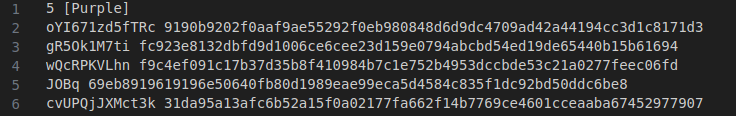
\includegraphics[height=3cm]{img/mdp.png}
    \caption{Données dans le fichier texte}
    \end{figure}
La profondeur correspond au nombre d'itérations du processus de compression et la couleur à la fonction de réduction qui vise à diminuer la probabilité de collision.

    \subsubsection{Récupération des données}
    L'objet BufferedReader est utilisé pour lire le fichier texte ligne par ligne, la première ligne est extraite pour obtenir la profondeur et les fonctions de réductions puis les lignes suivantes sont parcourues. BufferedReader est une classe Java utilisée pour la lecture de fichiers texte en mémoire tampon. Plutôt que de lire chaque caractère individuellement, ce qui peut être inefficace, le BufferedReader lit les données en blocs, ce qui réduit les appels coûteux. Cela en fait un choix idéal pour la lecture de fichiers texte ligne par ligne.
    
    \subsubsection{Comparaison des mots de passe}
    On utilise des fonctions de réduction pour obtenir le mot de passe. S'il n'y a aucune correspondance on effectue une recherche par couleur pour générer de nouveaux hash à partir du hash fourni jusqu’à trouver une correspondance ou atteindre la profondeur maximale.
    
    \subsubsection{Fonction de réduction}

    \begin{figure}[H]
    \centering
    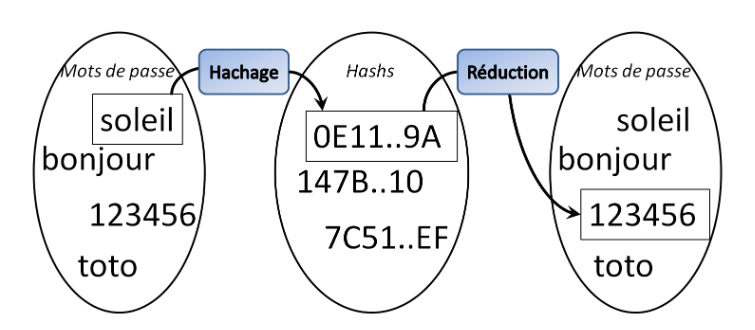
\includegraphics[height=7cm]{img/schema.png}
    \caption{Structure d’un maillon de chaîne}
    \end{figure}

    \begin{figure}[H]
    \centering
    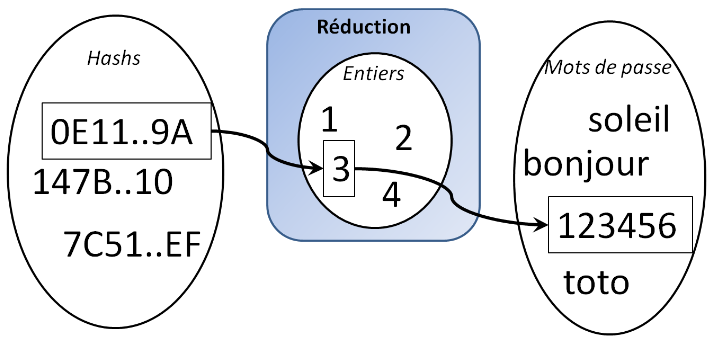
\includegraphics[height=7cm]{img/fonction_reduction.png}
    \caption{Décomposition d’une fonction de réduction}
    \end{figure}
    
    Les valeurs de hachage qui sont dans les tables arc-en-ciel sont créées à l’avance. Les personnes peuvent obtenir les tables arc-en-ciel et les utiliser pour chercher des mots de passe. Cependant, ces fichiers sont très volumineux donc on utilise une fonction de réduction pour éviter l’encombrement de l’espace de stockage. Dans une table arc-en-ciel une nouvelle valeur de hachage est générée à partir d'un mot de passe plusieurs fois, de sorte qu’une chaîne est créée. Dans la table finale seul le premier mot de passe et la dernière valeur de hachage de la chaîne apparaissent. Grâce a ses informations et en tenant compte des fonctions de réduction utilisées toutes les autres valeurs peuvent aussi être déterminées. La valeur de hachage à craquer est réduite de façon répétée et hachée selon les mêmes règles, chaque résultat intermédiaire étant comparé aux valeurs du tableau.

    Dans notre projet, nous avons 6 fonctions de réduction différentes (Orange, Blue, Purple, Yellow, Green et Red) chacune d'entre elles applique une réduction de hash différente. Par exemple "Orange" prend les caractères du hash aux positions impaires tandis que "Purple" prend les 32 premiers caractères du hash sur 64.
    
    \subsubsection{Interface graphique}
    L'interface graphique de notre application a été réalisée en utilisant Swing qui est une bibliothèque de composants graphiques avancée qui étend et améliore les fonctionnalités d'AWT.\newline
    \begin{figure}[H]
    \centering
    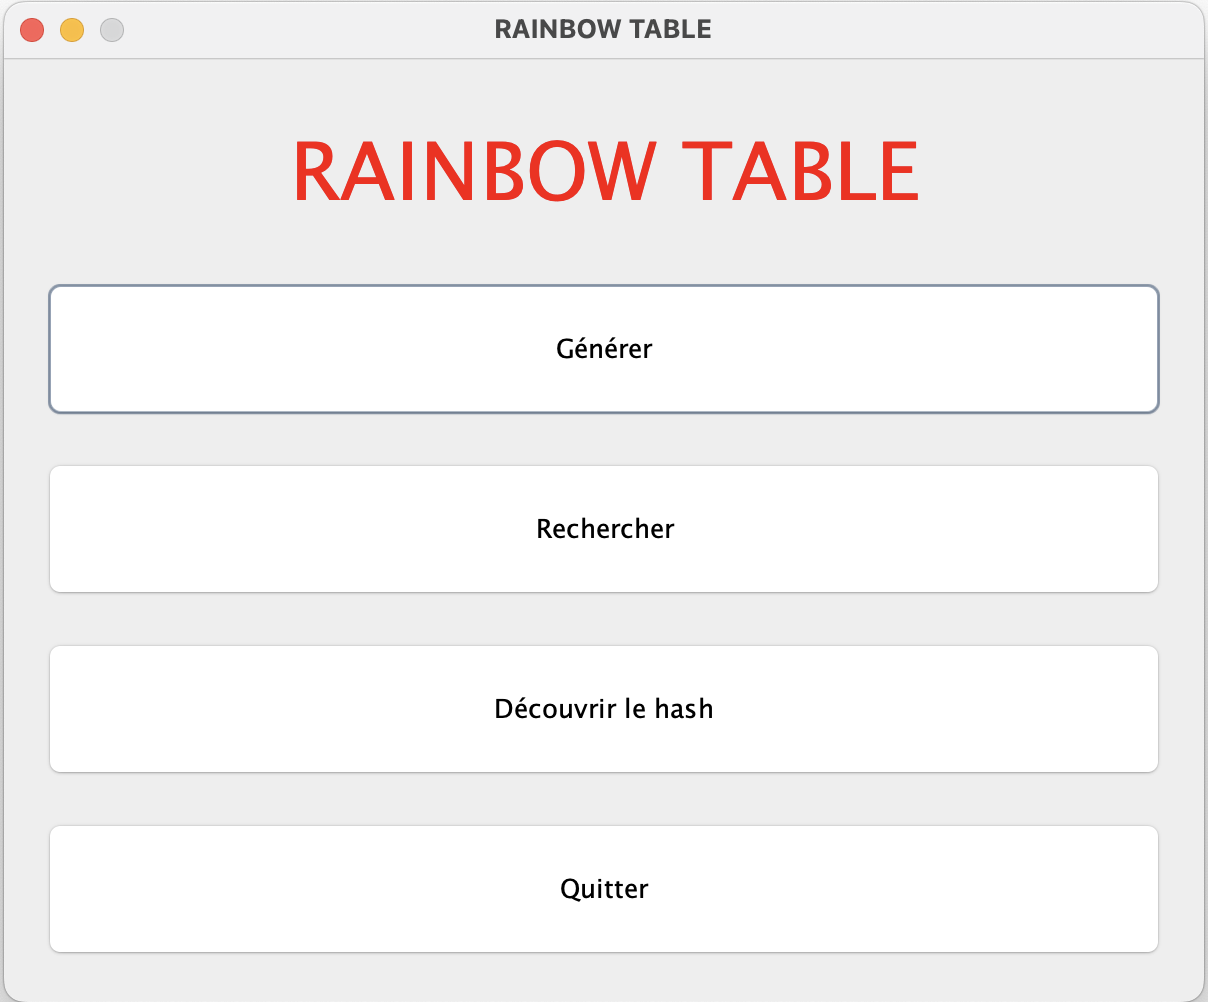
\includegraphics[height=11cm]{img/interface.png}
    \caption{Fenêtre principale de l'interface graphique}
    \end{figure}
     Si nous voulons générer une base de hash de mot passe, il faut cliquer sur le bouton "Générer". Puis de suivre les étapes suivantes ci dessous.
    \begin{figure}[H]
    \centering
    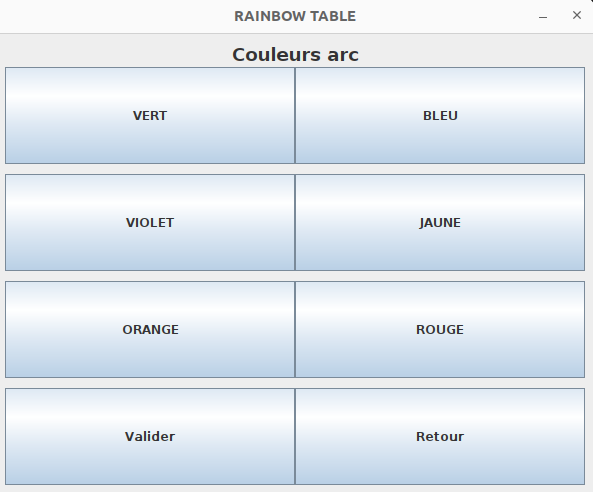
\includegraphics[height=10cm]{img/interface_couleurs.png}
    \caption{Fenêtre du choix des fonctions de réduction}
    \end{figure}
    Il faut désormais choisir les fonctions de réductions que l'on veux (minimum 1) en cliquant dessus.
    \begin{figure}[H]
    \centering
    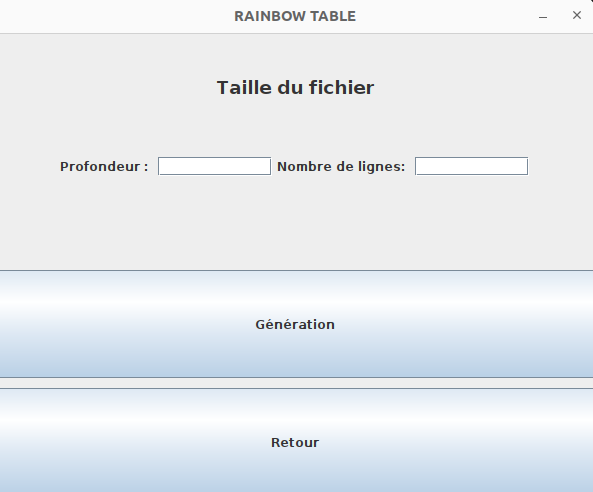
\includegraphics[height=10cm]{img/interface_taille.png}
    \caption{Fenêtre de la taille du fichier}
    \end{figure}
    Et enfin préciser la profondeur ainsi que le nombre de ligne. Une profondeur de 1000 associée à un nombre de lignes de 1000 générera au total (1000 x 1000) 1 000 000 de chaînes de hachage. Donc le fichier texte résultant occupera environ 80ko d'espace de stockage. De même, pour une profondeur de 500 avec un nombre de lignes de 500, le fichier texte totalisera une taille d'environ 40ko.
    \begin{figure}[H]
    \centering
    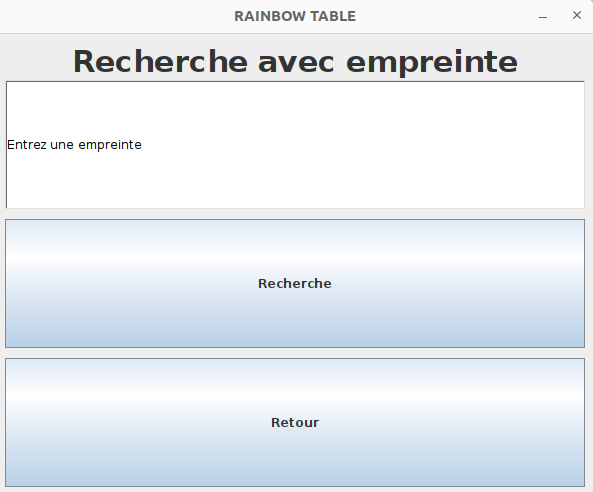
\includegraphics[height=9.5cm]{img/interface_recherche.png}
    \caption{Fenêtre de recherche d'empreinte}
    \end{figure}
    Si nous voulons rechercher un mot de passe grâce a son hash, il faut de cliquer sur le bouton "Rechercher" de la fenêtre principale puis d'entrer le hash dans la nouvelle fenêtre. Le hash entré doit être d'une longueur de 64 caractères puis enfin cliquer sur le bouton "Recherche". Il se peut que aucun mot de passe ne soit trouver.
    \begin{figure}[H]
    \centering
    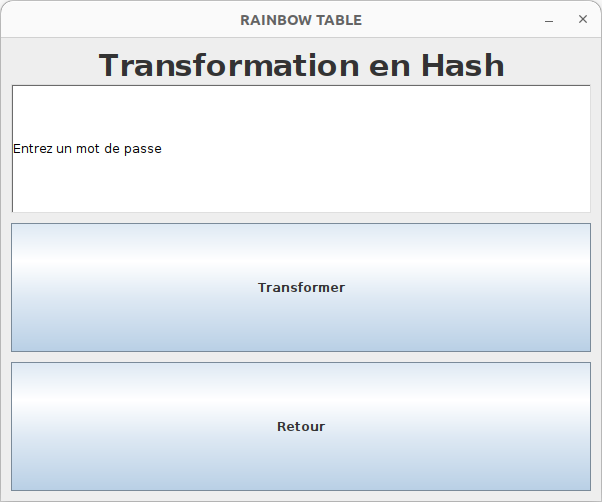
\includegraphics[height=9.5cm]{img/interface_transformation.png}
    \caption{Fenêtre de transformation en hash}
    \end{figure}
    Si nous voulons découvrir le hash d'un mot de passe, il faut cliquer sur le bouton "Découvrir le hash" de la fenêtre principale puis d'entrer le mot de passe dans la nouvelle fenêtre. Le hash entré doit être d'une longueur de 8 à 32 caractères.

\subsection{Organisation du projet}
\subsubsection{Répartition des tâches}
Pour la répartition des tâches, Awen s'est occupé de la génération des mots de passe et du stockage de leurs hash, Mael des fonctions de réduction ainsi que de la comparaison des hash, Valentin de la récupération des données dans un fichier et des tests unitaires puis pour finir Alexandre de l'interface graphique et du hachage des mots de passe. Le rapport et la soutenance ont étaient rédigé par Valentin.

\subsubsection{Logiciels utilisés}
Pour la gestion des versions du projet nous avons utilisé l'outil "Subversion" (SVN). SVN est un système de gestion de version centralisé, utilisé pour suivre et contrôler les modifications apportées à un ensemble de fichiers ou de dossiers au fil du temps. Ainsi que le site de la Forge de l'université de Caen, nous avons créé un groupe Discord pour la communication entre les différents membres du groupe. Pour la génération de diagramme nous avons utilisé le logiciel Dia. Pour l'écriture de ce rapport nous avons utilisé l'éditeur LaTeX en ligne Overleaf. Logiciel utilisé également pour la soutenance. Pour finir pour réaliser notre projet nous avons fait appel à un outil de construction de logiciel en Java nommé Ant permettant d'automatiser l'initialisation, la compilation, l'exécution, la génération de documentation, l'archivage au format JAR et l'exécution des tests. \\

\section{Éléments techniques}
\subsection{Description des paquetages non standards}
\subsubsection{Test unitaire}
Pour les tests unitaires, nous avons utilisé le framework de tests unitaires JUnit en version
3.8.2. Il est conçu pour le langage de programmation Java.
Il est utilisé pour faciliter le processus de test en permettant d’écrire des tests unitaires pour
vérifier la fonctionnalité des méthodes.
Ce framework fournit une série de classes et de méthodes pour écrire des tests unitaires, qui sont
des morceaux de code qui testent une méthode ou une classe individuelle. Nos tests unitaires
sont écrits à l’aide d’assertions, qui vérifient que le résultat d’une méthode ou l’initialisation
d’une variable est conforme à ce qui est attendu. Afin de réaliser les tests nous avons téléchargé
le fichier .jar de JUnit puis nous l’avons mis dans le répertoire "lib".\vspace{12pt}

Voici un aperçu des tests réalisés :\\

\begin{itemize}
    \item \textbf{Test de la classe HashCompare :} Ce test vérifie le bon fonctionnement de la comparaison de hachages. Nous avons vérifié que la création d'un hachage, la comparaison avec un hachage existant dans le fichier et la recherche d'un mot de passe associé à un hachage fonctionnent comme prévu.\newline
    
    \item \textbf{Test de la classe Menu :} Ce test garantit que le bouton de recherche dans le menu est initialisé correctement après la création de l'interface. Cela assure que l'interface est correctement configurée et prête à être utilisée.\newline
    
    \item \textbf{Test de la classe RainbowGUI :} Ce test vérifie si la fenêtre de l'interface graphique RainbowGUI est visible après sa création. Il s'assure que l'interface est rendue correctement et prête à être utilisée.\newline
    
    \item \textbf{Test de la classe Search :} Ce test vérifie si les fenêtres de recherche Search sont visibles, que ce soit avec un mot de passe trouvé ou non. Cela garantit que les fenêtres de recherche fonctionnent comme prévu.\newline
    
    \item \textbf{Test de la classe Rainbow :} Ce test vérifie le bon fonctionnement de la classe Rainbow en vérifiant si la méthode \texttt{ApplicationColor()} produit le résultat attendu. Cela assure que la logique de compression des couleurs fonctionne correctement.
\end{itemize}\vspace{12pt}

Voici ce qui est affiché dans le terminal après avoir exécuté les tests unitaires. Cela nous permet de connaître le nombre de tests réussis/échoués et de repérer les erreurs dans les tests. Nous remarquons que sur les 5 tests lancés aucun n'a échoué.

\begin{figure}[H]
\centering
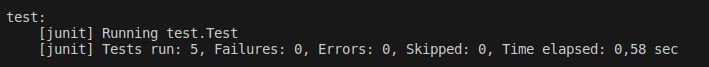
\includegraphics[height=1.7cm]{img/tests_unitaire.png}
\caption{Résultat des tests unitaires dans le terminal}
\end{figure}

Ces tests unitaires assurent une validation automatique du fonctionnement du code, ce qui contribue à sa fiabilité et à sa qualité.

\subsection{Descriptions des algorithmes}

\subsubsection{Génération de hash}

\begin{algorithm}
    \caption{Algorithme de création du hash SHA-256}
    \SetKwInOut{Output}{Sortie}
    \Output{Hash du mot de passe}
    $md \gets \text{MessageDigest.getInstance}("SHA-256")$\;
    $digest \gets md.digest(password.getBytes(StandardCharsets.UTF_8))$\;
    $sha \gets$ \textbf{new} StringBuilder$()$\;
    \For{$b$ \textbf{in} $digest$}{
        $sha.\text{append}(\text{String.format}("\%02x", b))$\;
    }
    \Return{$sha.\text{toString().toLowerCase()}$}\;
\end{algorithm}

Cet algorithme prend en entrée un mot de passe et retourne le hash SHA-256 correspondant. Il utilise l'algorithme de hachage SHA-256 fourni par la bibliothèque Java. Ensuite, il calcule le hash du mot de passe en convertissant d'abord le mot de passe en un tableau d'octets, puis en appliquant le hachage SHA-256. Le hash est converti en une chaîne de caractères hexadécimale pour le rendre lisible, puis il est retourné en minuscules.

\subsubsection{Génération d'un nouveau hash avec une réduction}

\begin{algorithm}
    \caption{Fonction hashIsNot}
    \SetKwInOut{Output}{Sortie}
    \KwIn{String $couleur$, String $hash$}
    \Output{Nouveau hash}
    $rainbow \gets$ \textbf{new} Rainbow$()$\;
    $hashReduc \gets rainbow.ApplicationColor(couleur, hash)$\;
    $generate \gets$ \textbf{new} Generate$(hashReduc)$\;
    $tmpMdp \gets generate.generatePassword()$\;
    $hashable \gets$ \textbf{new} Hash$(tmpMdp)$\;
    $hash \gets hashable.creeHash()$\;
    \KwRet{$hash$};
\end{algorithm}

Cet algorithme prend en entrée une couleur et un hash, puis il utilise la classe Rainbow pour appliquer une transformation de hash à l'aide de la couleur spécifiée. Ensuite, il génère un mot de passe à partir du hash réduit à l'aide de la classe Generate, puis recalcule le hash du mot de passe généré avec la classe Hash. Enfin, il renvoie le nouveau hash ainsi obtenu. Cette fonction est utilisée dans les méthodes de la classe HashCompare pour générer de nouveaux hash à partir de couleurs spécifiques.


\subsection{Descriptions des structures de données}
Pour stocker les couleurs, nous avons utilisé une ArrayList. C'est une structure de données dynamique dans Java, ce qui signifie qu'elle peut grandir ou rétrécir dynamiquement pendant l'exécution du programme. Chaque couleur est représentée par une chaîne de caractères (String). Cela permet aux classes d'accéder facilement aux différentes couleurs nécessaires pour compresser les mots de passe.\\\\Pour l'utiliser en Java nous devons l'importer avec la ligne : \\
\begin{lstlisting}[language=Java, numbers=left, basicstyle=\ttfamily\footnotesize, keywordstyle=\color{blue}\ttfamily, stringstyle=\color{red}\ttfamily, commentstyle=\color{green}\ttfamily,
numberstyle=\tiny, frame=single, linewidth=6cm]
import java.util.ArrayList;
\end{lstlisting}

Pour ajouter une couleur dans l'Arraylist nous devons faire par exemple :\\
\begin{lstlisting}[language=Java, numbers=left, basicstyle=\ttfamily\footnotesize, keywordstyle=\color{blue}\ttfamily, stringstyle=\color{red}\ttfamily, commentstyle=\color{green}\ttfamily,
numberstyle=\tiny, frame=single, linewidth=5.3cm]
tabCouleur.add("Green");
\end{lstlisting}

Pour récupérer une couleur dans l'ArrayList nous devons faire :\\
\begin{lstlisting}[language=Java, numbers=left, basicstyle=\ttfamily\footnotesize, keywordstyle=\color{blue}\ttfamily, stringstyle=\color{red}\ttfamily, commentstyle=\color{green}\ttfamily,
numberstyle=\tiny, frame=single, linewidth=6.6cm]
tabCouleur.get(indiceCouleur);
\end{lstlisting}

\subsection{Description des données}
\subsubsection{Données utilisateur}
\begin{itemize}
    \item Le hash
\end{itemize}
C'est le résultat l'application d'une fonction de hachage, c'est une valeur obtenue à partir de données d'entrée par exemple un mot de passe. Cette valeur est généralement de taille fixe, quelle que soit la taille des données d'origine. Les propriétés principales d'un bon algorithme de hachage incluent la résistance à la collision (deux mots de passe ne doivent pas générer le même hash) et la non-réversibilité (il doit être difficile de retrouver les données d'origine à partir du hash). Les fonctions de hachage sont utilisées pour sécuriser les données en cryptographie et pour vérifier l'intégrité des données.

\subsubsection{Données de configuration}
\begin{itemize}
    \item La profondeur
\end{itemize}
Elle fait référence au nombre d'itérations effectuées dans le processus de génération des rainbow tables. Chaque itération consiste à appliquer une fonction de hachage puis une fonction de réduction sur une valeur donnée, et ce processus est répété jusqu'à ce qu'une chaîne de longueur désirée soit obtenue. Plus la profondeur est grande, plus la rainbow tables est longue, ce qui peut potentiellement augmenter la capacité de recherche de mots de passe.\\

\begin{itemize}
    \item La longueur
\end{itemize}
Elle représente la taille des chaînes arc-en-ciel générées. Une longueur plus grande peut potentiellement augmenter la probabilité de couvrir un espace de recherche plus large pour les mots de passe.\\

\begin{itemize}
    \item Les couleurs
\end{itemize}
Elles font référence aux fonctions de réduction utilisées dans le processus de génération. Chaque couleur correspond à une fonction de réduction différente qui est appliquée à chaque itération pour transformer les valeurs hachées en nouvelles valeurs. Ces fonctions de réduction sont utilisées pour réduire la taille de l'espace de recherche des mots de passe et réduire les probabilités de collision comme dit précédemment.

\subsection{Se protéger des rainbow tables}
Pour se protéger contre les attaques utilisant des rainbow tables, il est essentiel d'adopter des pratiques de sécurité, notamment :\newline
\begin{itemize}
    \item Utiliser des fonctions de hachage robustes
\end{itemize}
Optez pour des algorithmes de hachage sécurisés et réputés comme SHA-256 ou SHA-3 plutôt que des algorithmes plus faibles comme MD5 ou SHA-1, qui sont vulnérables aux attaques par rainbow tables.\newline
\begin{itemize}
    \item Utiliser des techniques de salage (salt)
\end{itemize}
Le salage consiste à ajouter une chaîne aléatoire de données à chaque mot de passe avant de le hacher. Cela rend les attaques par rainbow tables beaucoup plus complexes, car chaque mot de passe haché est unique, même s'il s'agit du même mot de passe utilisateur.\newline
\begin{itemize}
    \item Implémenter des politiques de complexité de mot de passe
\end{itemize} 
Encouragez les utilisateurs à choisir des mots de passe longs, complexes et uniques, et imposez des politiques de renouvellement régulier des mots de passe pour réduire la probabilité qu'un mot de passe puisse être compromis et utilisé dans une attaque par rainbow tables.\newline
\begin{itemize}
    \item Surveiller et détecter les activités suspectes
\end{itemize}
Mettez en place des mécanismes de surveillance pour détecter les tentatives d'authentification anormales, ce qui peut indiquer une tentative d'utilisation de rainbow tables ou d'autres techniques d'attaque.

\section{Architecture du projet}
\subsection{Description des paquetages}
\begin{figure}[H]
\centering
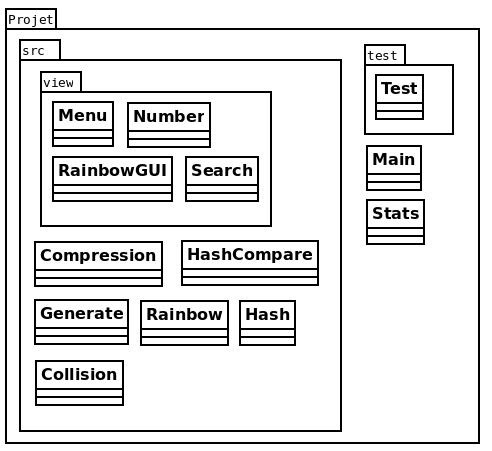
\includegraphics[height=10cm]{img/diagramme_paquetage.png}
\caption{Diagramme des paquetages}
\end{figure}
Ces paquetages sont divisés ainsi parce que nous avons eu la volonté de bien séparer l’aspect
visuel de l’aspect technique de notre projet. Les classes liées à l'interface utilisateur sont regroupées dans le paquetage view.

\subsection{Diagrammes des classes}

\begin{figure}[H]
\centering
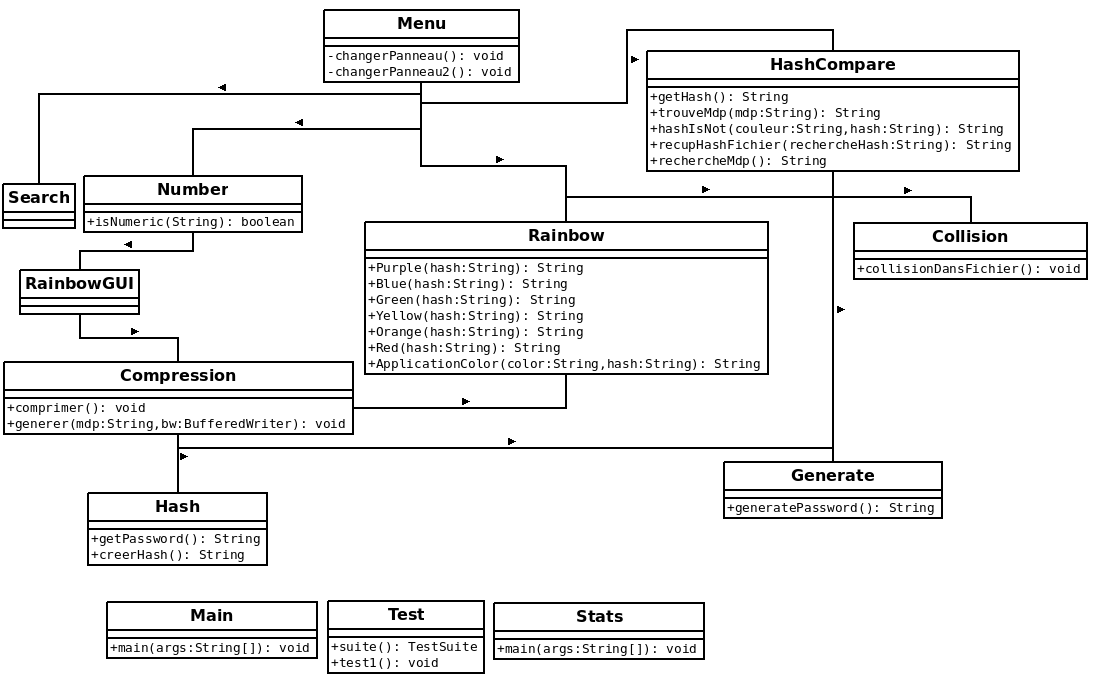
\includegraphics[height=11cm]{img/diagramme_classe.png}
\end{figure}
Les diagrammes des classes et des paquetages ont étaient fait grâce au logiciel de création de diagramme Dia. Il représente l'architecture logicielle de l'application. La classe Menu crée une interface utilisateur permettant à l'utilisateur d'interagir avec différentes fonctionnalités. Cette classe est associée à plusieurs autres classes telles que HashCompare, Number, Rainbow, et Search, qui sont responsables de différentes étapes du processus de génération et de recherche de mots de passe. La classe HashCompare effectue la comparaison d'empreintes et utilise la classe Rainbow pour générer des couleurs. La classe Number permet à l'utilisateur de spécifier la taille du fichier à générer, tandis que la classe RainbowGUI gère l'interface graphique pour afficher le processus de génération de mots de passe. La classe Search affiche le résultat de la recherche d'un mot de passe puis la classe Collision permet de vérifier si il y a une ou des collisions de hash.

\begin{figure}[H]
\centering
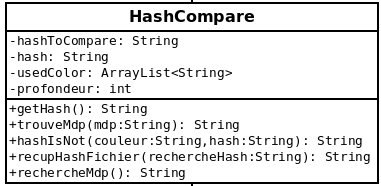
\includegraphics[height=5cm]{img/classe_hashcompare.png}
\caption{Diagramme de la classe HashCompare}
\end{figure}

Voyons plus en détail la classe HashCompare. Cette classe joue un rôle crucial dans la comparaison des hashs et la récupération des mots de passe associés. Elle est conçue pour interagir avec un fichier texte ("mdp.txt") contenant des associations de mots de passe et de hashs. La classe prend en attribut un hash, le hash à comparer et stocke également une liste de couleurs utilisées ainsi que la profondeur du processus de réduction de hash.\\ La méthode \texttt{trouveMdp} compare le hash fourni avec ceux stockés dans le fichier texte et retourne le mot de passe correspondant s'il existe. Elle utilise un processus de réduction de hash basé sur une liste de couleurs pour retrouver le mot de passe associé.\\ La méthode \texttt{hashIsNot} génère un nouveau hash en appliquant une réduction de hash basée sur une couleur spécifiée.\\ La méthode \texttt{recupHashFichier} recherche dans le fichier "mdp.txt" le mot de passe associé à un hash donné. Elle extrait les informations du fichier et utilise la méthode trouveMdp pour vérifier si le hash fourni correspond à celui de la ligne.\\ Et enfin la méthode \texttt{rechercheMdp} orchestre l'utilisation des méthodes précédentes pour rechercher le mot de passe associé à un hash donné. Elle commence par utiliser la méthode recupHashFichier pour récupérer le mot de passe correspondant au hash dans le fichier, puis, si nécessaire, génère de nouveaux hash à partir de différentes couleurs jusqu'à trouver le mot de passe correspondant.

\subsection{Chaînes de traitement}
Voici les étapes de la chaîne de traitement :\\
\begin{itemize}
    \item Menu principal
\end{itemize}
L'utilisateur interagit avec le menu principal pour choisir entre la génération de mots de passe avec leur hash associé, la recherche d'un mot de passe ainsi que découvrir le hash d'un mot de passe.\newline
\begin{itemize}
    \item Génération de mots de passe
\end{itemize}
L'utilisateur sélectionne cette option pour générer une table arc-en-ciel. Une fois l'option sélectionnée, l'interface lui permet de choisir les couleurs à inclure dans le processus de génération. L'utilisateur spécifie ensuite la taille du fichier à générer en termes de profondeur et de nombre de lignes. Une fois que toutes les informations sont fournies, le fichier de mots de passe est généré puis une interface indique à l'utilisateur que la génération est terminée.\newline
\begin{itemize}
    \item Recherche de mot de passe
\end{itemize}
L'utilisateur sélectionne cette option pour rechercher un mot de passe à partir d'une empreinte spécifiée. L'interface lui permet d'entrer une empreinte à rechercher. Une fois l'empreinte entrée, l'application compare cette empreinte aux empreintes existantes. Si un mot de passe correspondant est trouvé, il est affiché à l'utilisateur. Sinon, l'application indique à l'utilisateur que le mot de passe est introuvable.\newline
\begin{itemize}
    \item Découvrir le hash d'un mot de passe
\end{itemize}
L'utilisateur sélectionne cette option pour rechercher le hash d'un mot de passe à partir du mot de passe. L'interface lui permet d'entrer une empreinte à rechercher. Une fois le mot de passe entré, l'application affiche à l'utilisateur son hash.\newline
\begin{itemize}
    \item Retour et quitter
\end{itemize}
À chaque étape, l'utilisateur a la possibilité de retourner au menu principal pour effectuer une autre action ou de quitter l'application.

\section{Expérimentations}
\subsection{Cas d’utilisation}
\subsubsection{Documentation}

Pour générer la documentation, il suffit de se placer dans le dossier de la table arc-en-ciel puis d'écrire "ant javadoc" dans le terminal. Cela générera la documentation automatiquement à partir des contrats des classes et des méthodes et sera consultable directement sur un navigateur web. La documentation est stockée dans le dossier "doc".

\subsubsection{Lancement du jeu}

Afin de lancer l'interface graphique, il suffit d'écrire "ant run" dans le terminal qui s'occupera de créer le dossier build, de compiler les classes, de vérifier que les tests sont réussis puis d'exécuter la classe principale. Ensuite, vous pourrez choisir entre la génération d'une rainbow table, la recherche de mot de passe ou la découverte du hash d'un mot de passe selon vos besoins. Cela est possible grâce au fichier build.xml qui définit les différentes tâches à exécuter lors de la commande "ant run". L'utilisation de "ant run" simplifie le processus en automatisant les étapes nécessaires à l'exécution de l'application, ce qui facilite grandement son utilisation pour l'utilisateur final. 

\subsection{Résultats quantifiables}
Profondeur 1000, longueur 1
\begin{itemize}
    \item Temps de compression : 279 ms
    \item Temps de recherche : 1097 ms
    \item Taille : 102 octets
\end{itemize}

Profondeur 10, longueur 10
\begin{itemize}
    \item Temps de compression : 152 ms
    \item Temps de recherche : 591 ms
    \item Taille : 831 octets
\end{itemize}

Profondeur 10, longueur 100
\begin{itemize}
    \item Temps de compression : 109 ms
    \item Temps de recherche : 398 ms
    \item Taille : 8169 octets
\end{itemize}

Profondeur 1, longueur 1000
\begin{itemize}
    \item Temps de compression : 89 ms
    \item Temps de recherche : 301 ms
    \item Taille : 81000 octets
\end{itemize}
\newpage
Voici les résultats sous forme de graphique :
\begin{figure}[H]
\centering
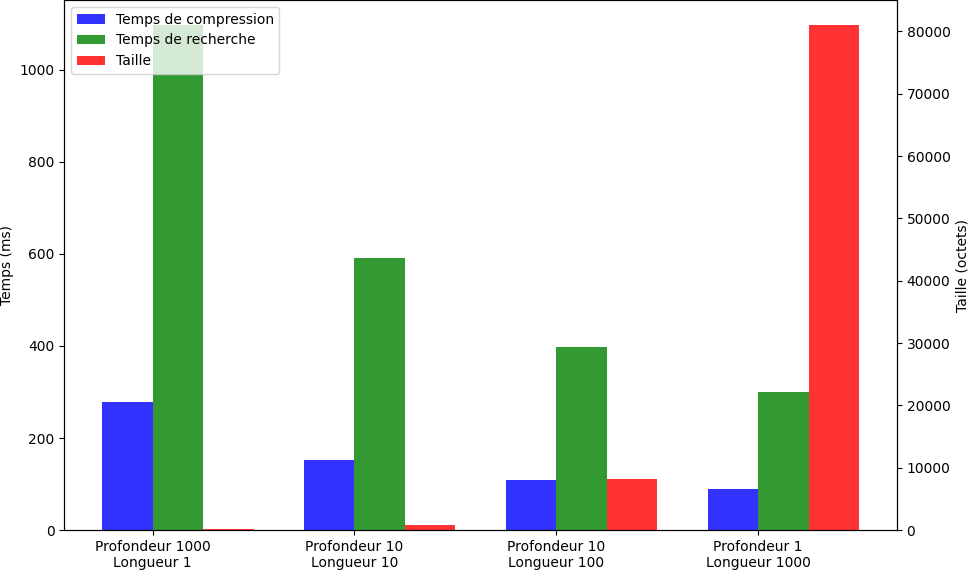
\includegraphics[height=10cm]{img/graphique.png}
\caption{Graphique représentant le temps de compression, de recherche et la taille en fonction de la profondeur et de la longueur}
\end{figure}

\subsection{Analyse des résultats}
Chaque barre du graphique représente une mesure pour une profondeur et une longueur spécifique. Les valeurs sur l'axe des x indiquent la longueur et la profondeur, tandis que les valeurs sur l'axe des y représentent le temps nécessaire pour effectuer les opérations, mesuré en millisecondes (ms) pour les temps de compression et de recherche, et en octets pour la taille. Ainsi, ce graphique permet de visualiser l'évolution du temps de compression, du temps de recherche et de la taille en fonction de la longueur pour différentes profondeurs, offrant ainsi des informations précieuses pour l'optimisation des performances.\newline

D'après les données fournies, la configuration optimale semble être une profondeur de 10 et une longueur de 100. Cette configuration offre un bon compromis entre le temps de compression, le temps de recherche et la taille de la table. Augmenter la profondeur augmente le temps de compression et de recherche mais diminue la taille de la table. Augmenter la longueur diminue le temps de compression et de recherche mais augmente la taille de la table. Le choix de la configuration optimale dépendra de vos besoins spécifiques.

\section{Conclusion}

\subsection{Récapitulatif de la problématique et de la réalisation}
Notre objectif principal était de concevoir et de mettre en œuvre une table arc-en-ciel fonctionnelle et optimisée en utilisant le langage de programmation Java. Pour ce faire, nous avons dû relever plusieurs défis, notamment la génération de mots de passe, le stockage des hashs associés et la mise en place d'une interface graphique. Ce projet nous a permis d'approfondir nos connaissances en programmation Java, en algorithmique et en gestion de projet. 

\subsection{Récapitulatif des résultats}
Le temps nécessaire pour générer une rainbow tables avec une longueur de 1 et une profondeur de 1000 serait d'environ 279 ms avec une taille de 102 octets, tandis que pour une chaîne avec une longueur de 10 et une profondeur de 10, ce temps serait réduit à environ 152 ms avec une taille de 831 octets.

\subsection{Propositions d’améliorations}
Nous avons plusieurs idées pour d'éventuelles améliorations :
\begin{description}
    \item [Ajouter de nouveaux tests unitaires] : Nous pourrions étendre notre suite de tests unitaires pour couvrir davantage de cas d'utilisation et garantir une plus grande robustesse de notre application. Cela permettrait de détecter plus facilement d'éventuels bugs ou erreurs de fonctionnement.
    \item [Version de JUnit] : Envisager de passer à la dernière version de JUnit, la 5.9.2 au lieu de la 3.8.2 afin de bénéficier des dernières fonctionnalités et améliorations de JUnit, ainsi que de bénéficier d’un support actif et de correctifs de bogues.
    \item [Implémenter des optimisations connues] : Il existe plusieurs techniques d'optimisation des tables arc-en-ciel, telles que l'utilisation de chaînes de Markov ou de fonctions de réduction plus complexes. Nous pourrions améliorer significativement les performances de notre application.
    \item [Ajouter un système de logging] : L'intégration d'un système de logging nous permettrait de suivre et d'enregistrer les actions et les événements importants se produisant lors de l'exécution de l'application. Cela faciliterait le processus de débogage en fournissant des informations détaillées sur les erreurs, les avertissements et les activités ce qui serait utile pour diagnostiquer et résoudre les problèmes.
    \item [Ajouter la prise en charge de nouveaux algorithme de hachage] : Pour rendre notre application plus polyvalente et adaptable, nous pourrions étendre son support pour inclure une variété d'algorithmes de hachage supplémentaires. Cela offrirait aux utilisateurs la possibilité de choisir parmi une gamme plus large d'options de hachage, en fonction de leurs besoins spécifiques.
    \item [Implémenter une interface de statistique] : Il serait intéressant d’implémenter des options pour l’analyse et la visualisation des statistiques directement sur l'interface. Par exemple, il pourrait être possible d’afficher des graphiques pour visualiser l’efficacité des tables en fonction du temps, de la longueur, de la profondeur et des fonctions de réductions ce qui permettrait d’avoir des résultats encore plus concrets.
\end{description}
En mettant en œuvre ces propositions, nous pourrions rendre notre projet plus performant, plus robuste et plus adaptable aux besoins des utilisateurs.

\end{document}